
%------------------------------------------------
\section{Vulnérabilités}
%------------------------------------------------

\begin{frame}
\frametitle{Types de vulnérabilités}

Il existe de nombreux types de vulnérabilités, mais il est pratique de les lister par type d'impact possibles:
\begin{itemize}
 \item Denial Of Service % Bash ForkBomb
 \item Information Leakage % Heartbleed
 \item Man In The Middle % Lenovo Superfish
 \item Privilege Escalation % Rowhammer
 \item Remote Code Execution % Shellshock

\end{itemize}

\end{frame}

\subsection{Denial Of Service}
\begin{frame}
\frametitle{Exemple: Fork Bomb}

\begin{center}
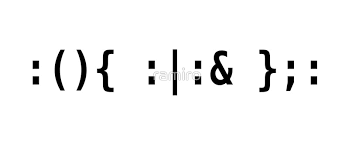
\includegraphics[scale=0.55]{res/bash_fork}
\end{center}

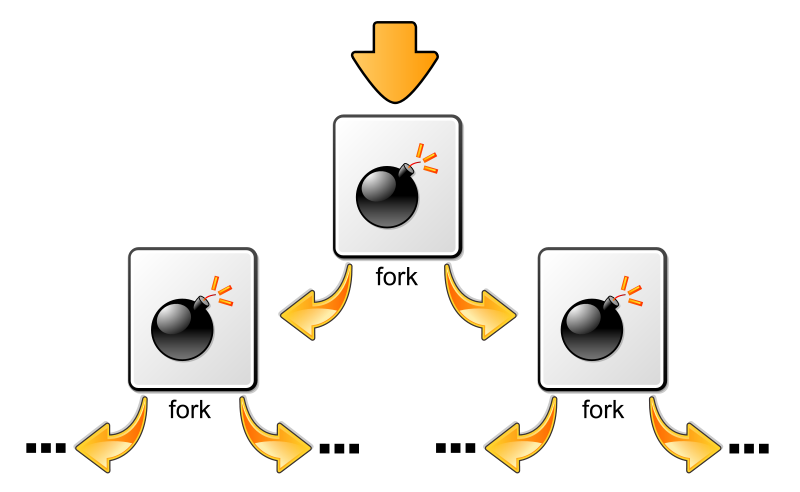
\includegraphics[scale=0.24]{res/fork_bomb}
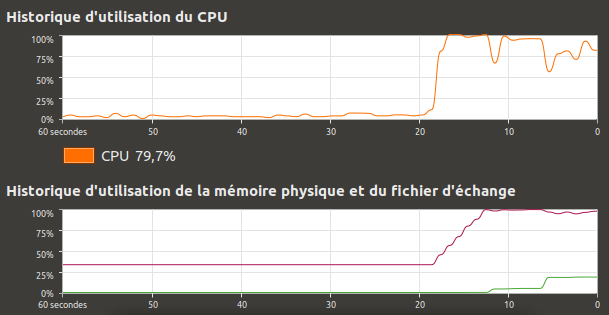
\includegraphics[scale=0.24]{res/DoS}

\end{frame}




\subsection{Information Leakage}
\begin{frame}
\frametitle{Exemple: Heartbleed}

\begin{center}
    Heartbleed\\
    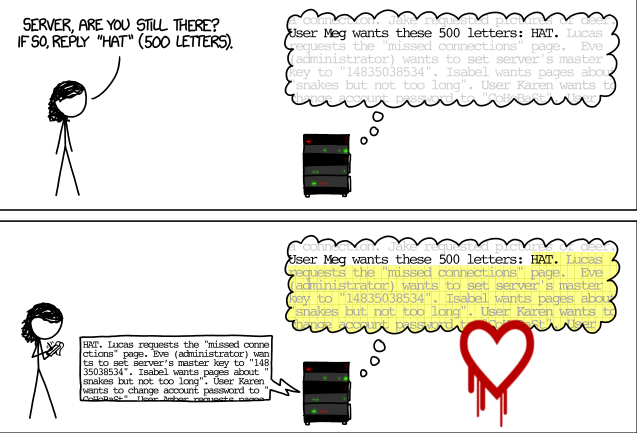
\includegraphics[scale=0.44]{res/heartbleed_explanation}
\end{center}


\end{frame}


\note{

     \href{https://arstechnica.com/security/2014/04/critical-crypto-bug-in-openssl-opens-two-thirds-of-the-web-to-eavesdropping/}{\beamergotobutton{
        Heartbleed: Ars Technica Article
    }}\\

    \href{https://xkcd.com/1354/}{\beamergotobutton{
        Heartbleed: xkcd explanation
    }}

}

\subsection{Man In The Middle}
\begin{frame}
\frametitle{Exemple: Superfish}

\begin{center}
    Lenovo's Massive Fuckup\\
    \vspace{3em}
    
\includegraphics[scale=0.24]{res/superfish}
\end{center}


\end{frame}

\note{

    \href{https://arstechnica.com/security/2015/02/lenovo-pcs-ship-with-man-in-the-middle-adware-that-breaks-https-connections/}{\beamergotobutton{
        Why I don't like Lenovo
    }}

}






\subsection{Privilege Escalation}
\begin{frame}
\frametitle{Exemple: Rowhammer}

\begin{center}
    Physical attack on DRAM memory\\
    \vspace{2em}
    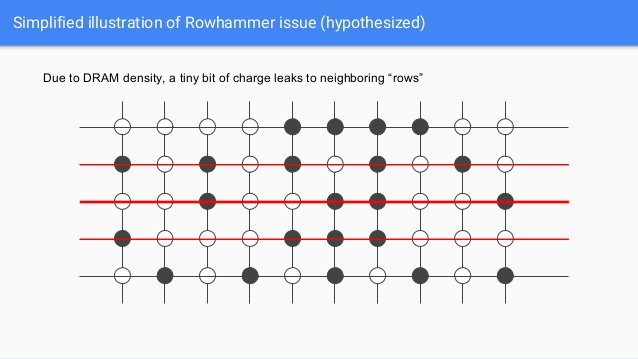
\includegraphics[scale=0.24]{res/rowhammer}
\end{center}
\begin{itemize}
    \item En changeant les valeurs d'une page de mémoire répétitivement, il est possible de faire changer la valeur de Bits dans la page d'à côté.
    \item Cela peut permettre à un programme tournant avec des privilèges utilisateurs d'obtenir les privilèges de root.
\end{itemize}
\end{frame}

\note{

    \href{https://googleprojectzero.blogspot.fr/2015/03/exploiting-dram-rowhammer-bug-to-gain.html}{\beamergotobutton{
        Project Zero writeup on Rowhammer
    }}

}




\subsection{Remote Code Execution}
\begin{frame}
\frametitle{Exemple: Shellshock}

\begin{center}
    24 Septembre 2014\\
    Une des pires vulnérabilités de tout les temps.\\
    \vspace{2em}
    
\includegraphics[scale=0.54]{res/shellshock}
    \begin{itemize}
        \item Permet d'exécuter du code arbitraire sur des serveurs web
        \item Dans les jours suivant l'annonce, un scan automatique massif d'internet était en cours pour compromettre des serveurs
    \end{itemize}
\end{center}
\end{frame}



\note{
    \href{https://arstechnica.com/security/2014/09/bug-in-bash-shell-creates-big-security-hole-on-anything-with-nix-in-it/}{\beamergotobutton{
        Ars Technica's article on Shellshock
    }}


}


